\documentclass[tikz,border=2pt]{standalone}
\usepackage{tikz}
\usetikzlibrary{calc}

\begin{document}
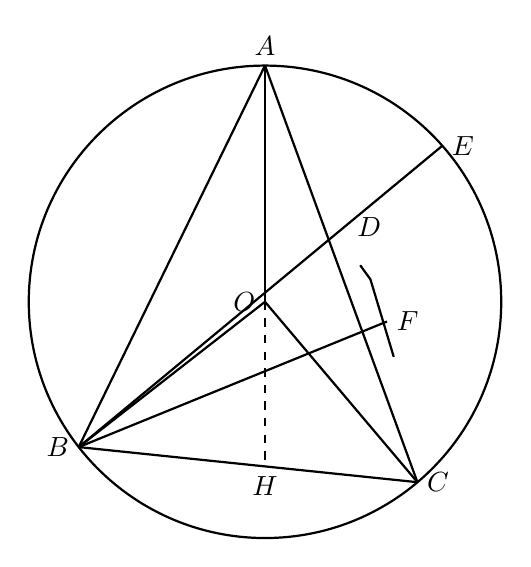
\begin{tikzpicture}[scale=1]

% Circle
\draw[line width=0.8pt] (0,0) circle (3);

% Key points
\coordinate (O) at (0,0);
\coordinate (A) at (0,3);
\coordinate (H) at (0,-2.1);
\coordinate (B) at (-2.366,-1.845);
\coordinate (C) at (1.936,-2.291);
\coordinate (E) at (2.25,1.98);

% Auxiliary points
\coordinate (D) at (1.05,0.95);
\coordinate (F) at (1.55,-0.25);

% Main triangle and chords
\draw[line width=0.8pt] (A) -- (B);
\draw[line width=0.8pt] (A) -- (C);
\draw[line width=0.8pt] (B) -- (C);
\draw[line width=0.8pt] (B) -- (E);

% Radii / inner segments
\draw[line width=0.8pt] (O) -- (B);
\draw[line width=0.8pt] (O) -- (C);
\draw[line width=0.8pt] (B) -- (F);

% Edited segment: AO changed from dashed to solid
\draw[line width=0.8pt] (A) -- (O);

% Remaining dashed segment
\draw[dashed,line width=0.8pt] (O) -- (H);

% Right-angle mark near F
\coordinate (P) at ($(F)!0.22!(A)$);
\coordinate (Q) at ($(F)!0.22!(C)$);
\coordinate (R) at ($(P)+(0.13,-0.18)$);
\draw[line width=0.8pt] (P) -- (R) -- (Q);

% Labels
\node[above] at (A) {$A$};
\node[left] at (B) {$B$};
\node[right] at (C) {$C$};
\node[right] at (E) {$E$};
\node[left] at (O) {$O$};
\node[below] at (H) {$H$};
\node[right] at (D) {$D$};
\node[right] at (F) {$F$};

\end{tikzpicture}
\end{document}
